\section{Frontend Architecture e User Experience}
\label{sec:frontend_ux}

\subsection{Architettura della Single Page Application (React 18 + Vite)}
Il client web di TEPO è sviluppato come Single Page Application (SPA) reattiva impiegando la libreria \textbf{React 18} con linguaggio \textbf{TypeScript 5.5} e build tool \textbf{Vite 5}. L'architettura è stata progettata per garantire latenza minima nelle interazioni, totale indipendenza dello stato client durante l'esplorazione dei dati e conformità rigorosa ai contratti DTO esposti dal backend.

\subsubsection{Organizzazione Modulare dei Componenti}
Il codice sorgente dell'interfaccia utente è strutturato nelle seguenti directory logiche:
\begin{itemize}[leftmargin=1.5em, itemsep=0.2em]
    \item \textbf{\texttt{src/components/shell/}:} Include l'impalcatura strutturale dell'applicazione (\texttt{AppShell}), la barra laterale di navigazione (\texttt{SideNav}), la striscia di stato permanente con dichiarazione del dataset demo (\texttt{StatusBand}), il selettore del tema (\texttt{ThemeToggle}) e la tavolozza dei comandi (\texttt{CommandPalette}).
    \item \textbf{\texttt{src/components/ui/}:} Fornisce le primitive di interfaccia riutilizzabili (\texttt{primitives.tsx}, \texttt{Modal.tsx}, \texttt{Toast.tsx}, \texttt{Icon.tsx}, \texttt{SortableTh.tsx}), concepite senza librerie CSS esterne pesanti per massimizzare la velocità di rendering.
    \item \textbf{\texttt{src/components/charts/}:} Implementa componenti grafici vettoriali SVG nativi e accessibili (curve di efficienza cumulativa, diagrammi a barre e matrici di calore), dotati di descrizioni testuali alternative per screen reader.
    \item \textbf{\texttt{src/services/scenarioStore.ts}:} Incapsula la gestione dello stato client, sincronizzando in memoria locale (\texttt{LocalStorage}) le selezioni correnti, lo storico dei risultati e gli slot di confronto \emph{Slot A} e \emph{Slot B}.
    \item \textbf{\texttt{src/hooks/}:} Custom hook specializzati per la gestione asincrona delle chiamate REST (\texttt{useAsyncData}), il ciclo di vita della sessione (\texttt{useSession}) e la commutazione dinamica del tema visivo (\texttt{useTheme}).
\end{itemize}

\subsection{Design System Civico ``Strumento Civico'' e Accessibilità}
L'identità visiva di TEPO, denominata ``Strumento Civico'', risponde alle specifiche esigenze operative di un ufficio tecnico comunale: chiarezza tipografica, alta densità di informazioni pertinenti, assenza di elementi decorativi superflui e piena neutralità algoritmica.

\subsubsection{Doppio Registro Visivo: Relazione e Sala Operativa}
Per adattarsi ai molteplici contesti d'uso della Pubblica Amministrazione, TEPO supporta due registri cromatici nativi commutabili istantaneamente:
\begin{itemize}[leftmargin=1.5em, itemsep=0.2em]
    \item \textbf{Tema Relazione (Chiaro):} Ottimizzato per la lettura diurna su monitor d'ufficio, la proiezione durante riunioni istituzionali o consigli comunali e la stampa cartacea di relazioni tecniche allegate a delibere di spesa.
    \item \textbf{Tema Sala Operativa (Scuro ad Alto Contrasto):} Progettato per sessioni analitiche continuative e prolungate, riducendo l'affaticamento visivo dell'operatore tecnico attraverso sfondi antracite desaturati e bordi ad alta definizione.
\end{itemize}

\subsubsection{Conformità alle Linee Guida WCAG 2.1 Livello AA}
L'interfaccia rispetta rigorosamente i requisiti internazionali di accessibilità web:
\begin{enumerate}[leftmargin=1.4em, itemsep=0.2em]
    \item \textbf{Rapporto di Contrasto Cromatico:} Tutte le combinazioni di testo e sfondo garantiscono un contrasto minimo superiore a $4.5:1$ per il corpo del testo e a $3:1$ per gli elementi grafici interattivi e le intestazioni.
    \item \textbf{Navigabilità Integrale da Tastiera:} L'intera applicazione è utilizzabile senza l'ausilio del mouse; l'ordine dei focus (\texttt{tabindex}) rispetta la gerarchia visiva ed evidenzia chiaramente l'elemento attivo tramite un anello di selezione (\emph{focus ring}) cromaticamente marcato.
    \item \textbf{Compatibilità Screen Reader:} I pulsanti e i controlli interattivi sono corredati da etichette semantiche esplicite (\texttt{aria-label}, \texttt{aria-expanded}, \texttt{role="status"}), permettendo ai lettori di schermo di comunicare fedelmente lo stato delle elaborazioni e dei filtri attivi.
    \item \textbf{Responsive Design:} Il layout adotta un'impostazione fluida garantita da Flexbox e CSS Grid, offrendo una fruizione ottimale da risoluzioni smartphone (320px) fino a monitor desktop ultrawide (1920px).
\end{enumerate}

\subsubsection{Tavolozza dei Comandi Rapidi (\texttt{CommandPalette})}
Per massimizzare la produttività degli utenti esperti, la shell integra una tavolozza comandi attivabile globalmente tramite la combinazione di tasti \texttt{Ctrl+K} (oppure \texttt{Cmd+K} su macOS). Essa consente di ricercare istantaneamente qualsiasi edificio per nome o indirizzo, navigare verso le viste decisionali, commutare il tema visivo ed eseguire l'ottimizzazione senza distogliere le mani dalla tastiera.

\subsection{Analisi Dettagliata delle Viste Operative dell'Applicazione}
Il percorso decisionale di TEPO si articola in nove viste operative specializzate, analizzate di seguito con riferimento agli screenshot reali estratti dal sistema in esecuzione.

\subsubsection{1. Dashboard di Controllo}
Costituisce la pagina iniziale del sistema. Espone un cruscotto sintetico con quattro indicatori chiave (KPI) sul patrimonio analizzato: numero totale di edifici (100), interventi disponibili (300), potenziale di risparmio energetico complessivo e scorciatoie per l'avvio immediato di una nuova ottimizzazione.
La Figura~\ref{fig:screens_dashboard} pone a confronto la resa visiva della Dashboard nel tema chiaro \emph{Relazione} e nel tema scuro \emph{Sala Operativa}.

\begin{figure}[H]
    \centering
    \begin{subfigure}[t]{0.48\linewidth}
        \centering
        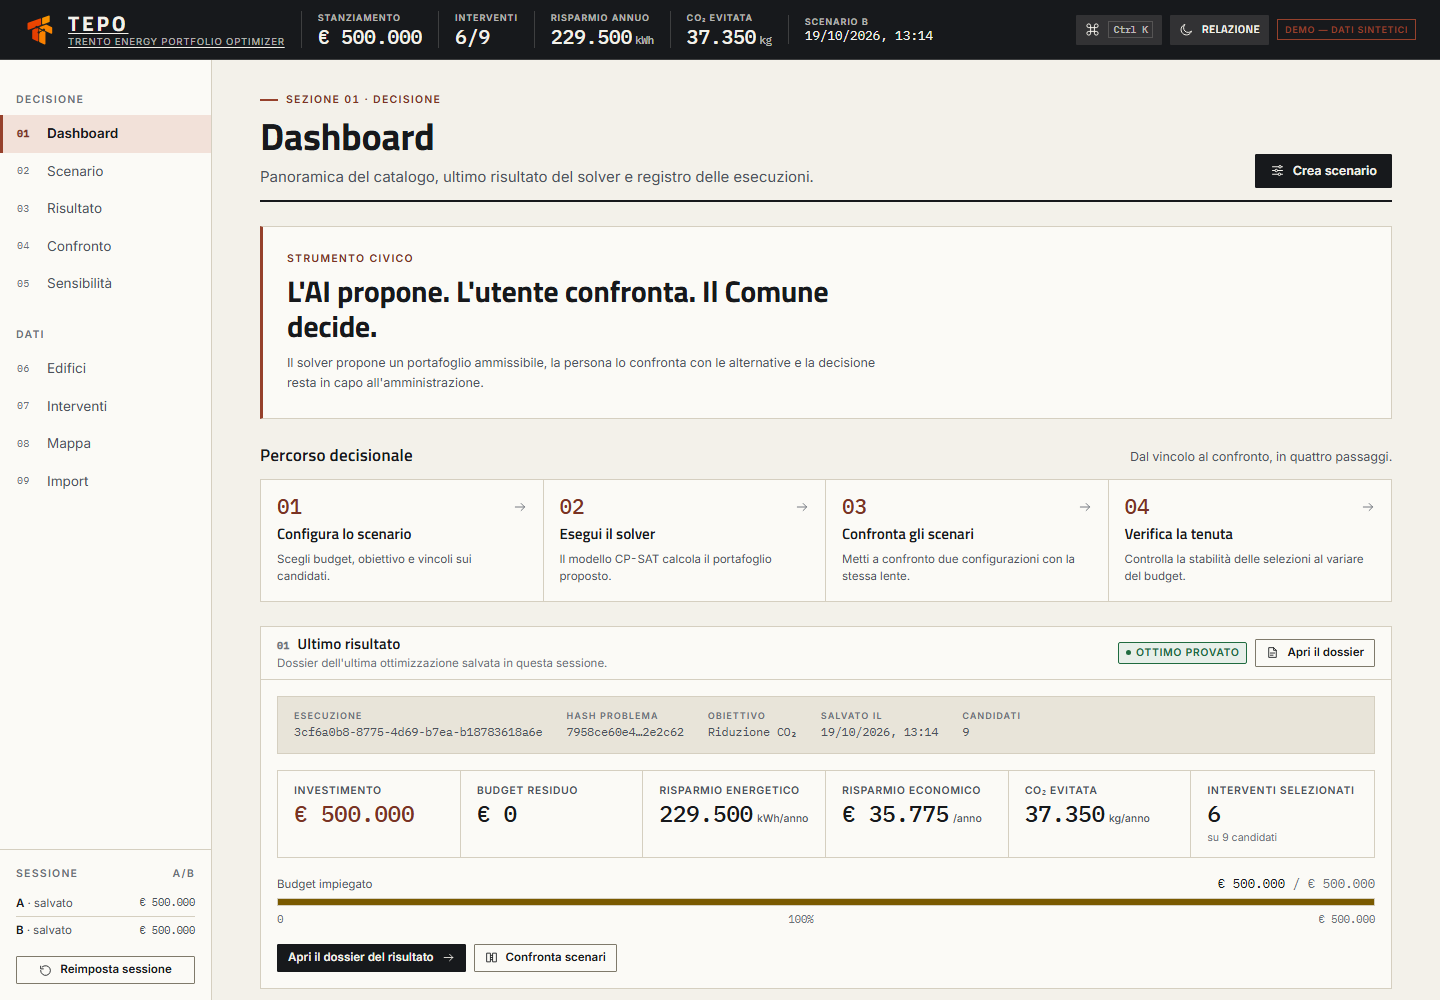
\includegraphics[width=\linewidth]{img/dashboard-relazione.png}
        \caption{Dashboard nel registro visivo ``Relazione'' (chiaro).}
        \label{fig:dash_rel}
    \end{subfigure}
    \hfill
    \begin{subfigure}[t]{0.48\linewidth}
        \centering
        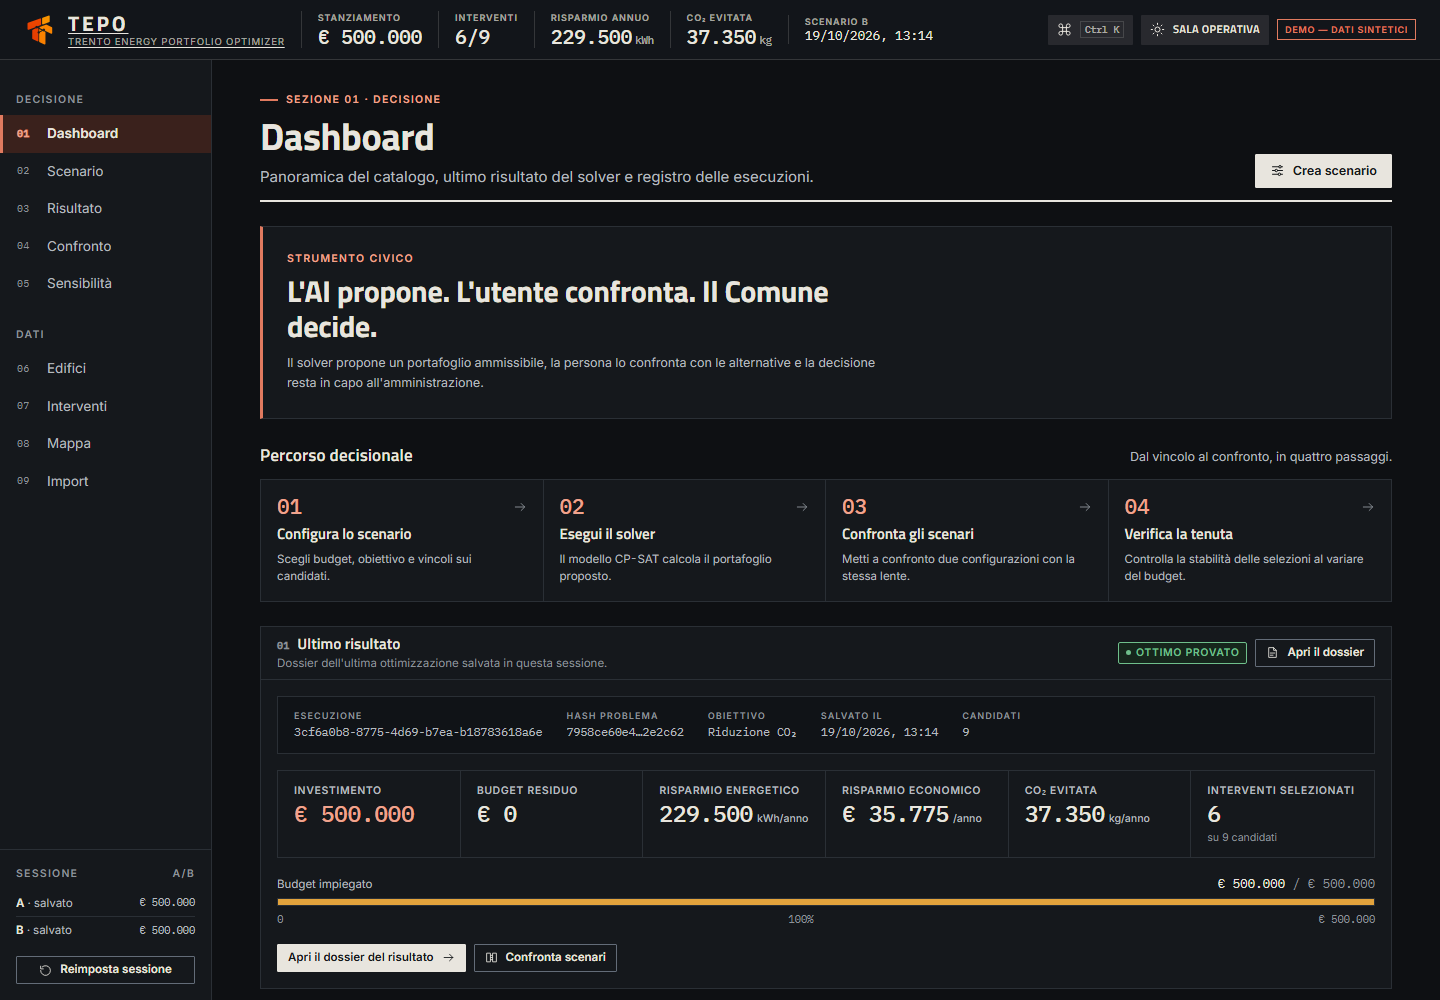
\includegraphics[width=\linewidth]{img/dashboard-sala-operativa.png}
        \caption{Dashboard nel registro ``Sala Operativa'' (scuro).}
        \label{fig:dash_op}
    \end{subfigure}
    \caption{Dashboard di controllo di TEPO nei due temi operativi.}
    \label{fig:screens_dashboard}
\end{figure}

\subsubsection{2. Mappa Cartografica Georeferenziata}
La vista \texttt{MapPage} integra la mappa del territorio comunale di Trento tramite la libreria Leaflet (Figura~\ref{fig:screen_map}). Ciascun edificio è localizzato con precisione e corredato da un indicatore circolare la cui ampiezza e colorazione rispecchiano la concentrazione degli interventi e il volume di investimento. Al click su un marcatore, si apre un popup informativo con i dati catastali e il link diretto alla scheda dell'edificio.

\begin{figure}[H]
    \centering
    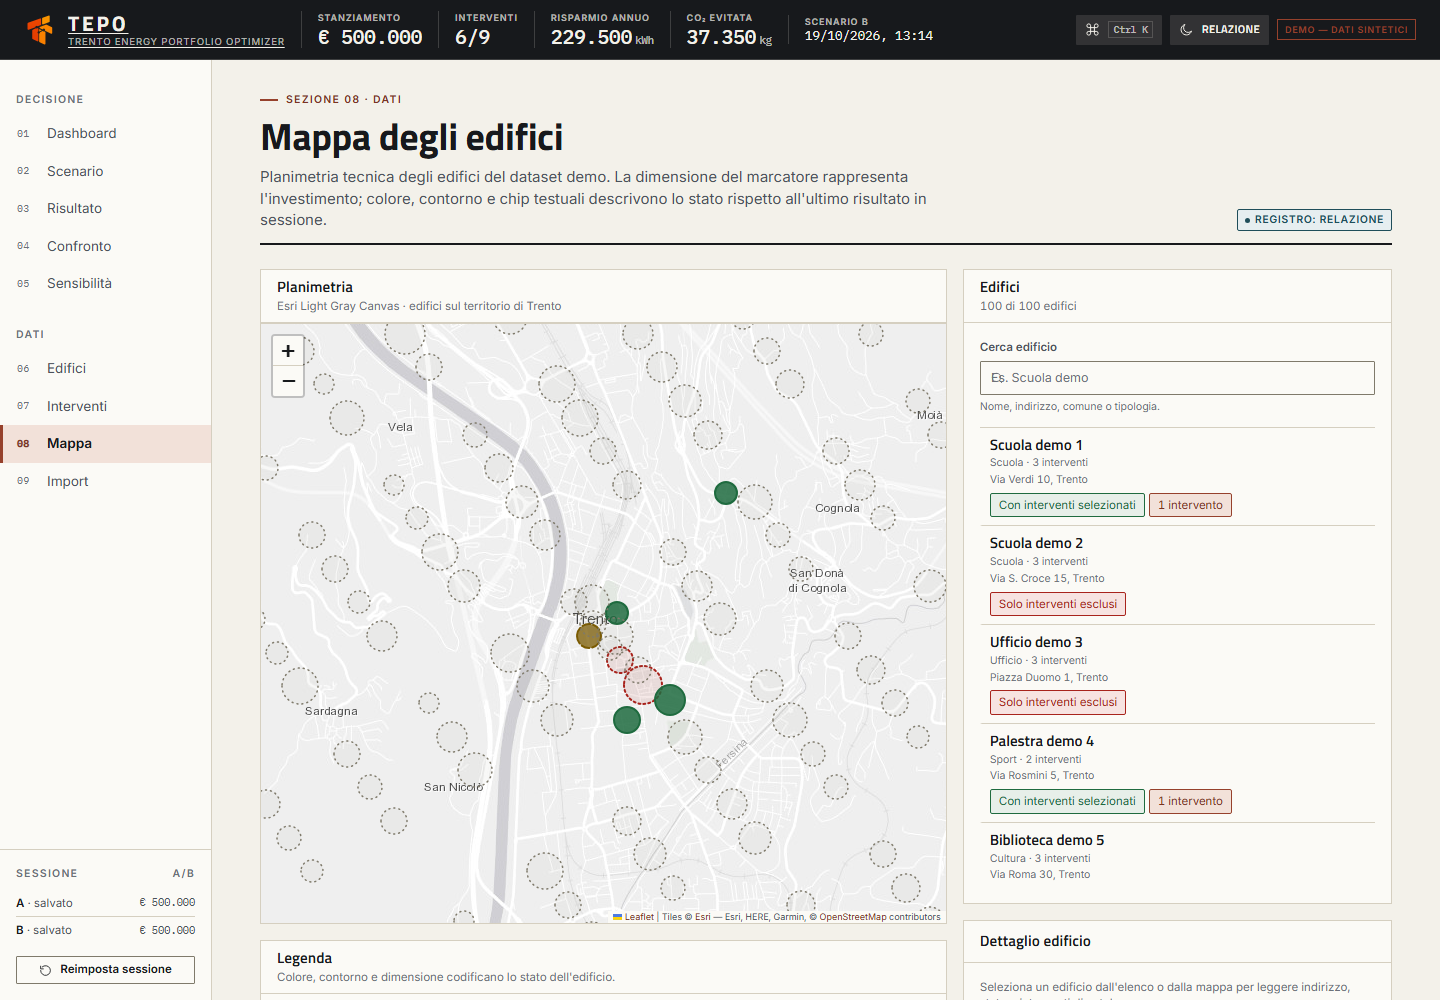
\includegraphics[width=0.85\linewidth]{img/mappa.png}
    \caption{Cartografia georeferenziata degli edifici di Trento su mappa interattiva.}
    \label{fig:screen_map}
\end{figure}

\subsubsection{3. Cataloghi degli Edifici e degli Interventi}
Le viste \texttt{BuildingsPage} (Figura~\ref{fig:screen_edifici}) e \texttt{InterventionsPage} (Figura~\ref{fig:screen_interventi}) consentono l'esplorazione tabellare analitica del patrimonio. Entrambe le tabelle offrono ordinamento multi-colonna, ricerca testuale in tempo reale, filtri per tipologia e badge espliciti sulla provenienza sintetica del dato.

\begin{figure}[H]
    \centering
    \begin{subfigure}[t]{0.48\linewidth}
        \centering
        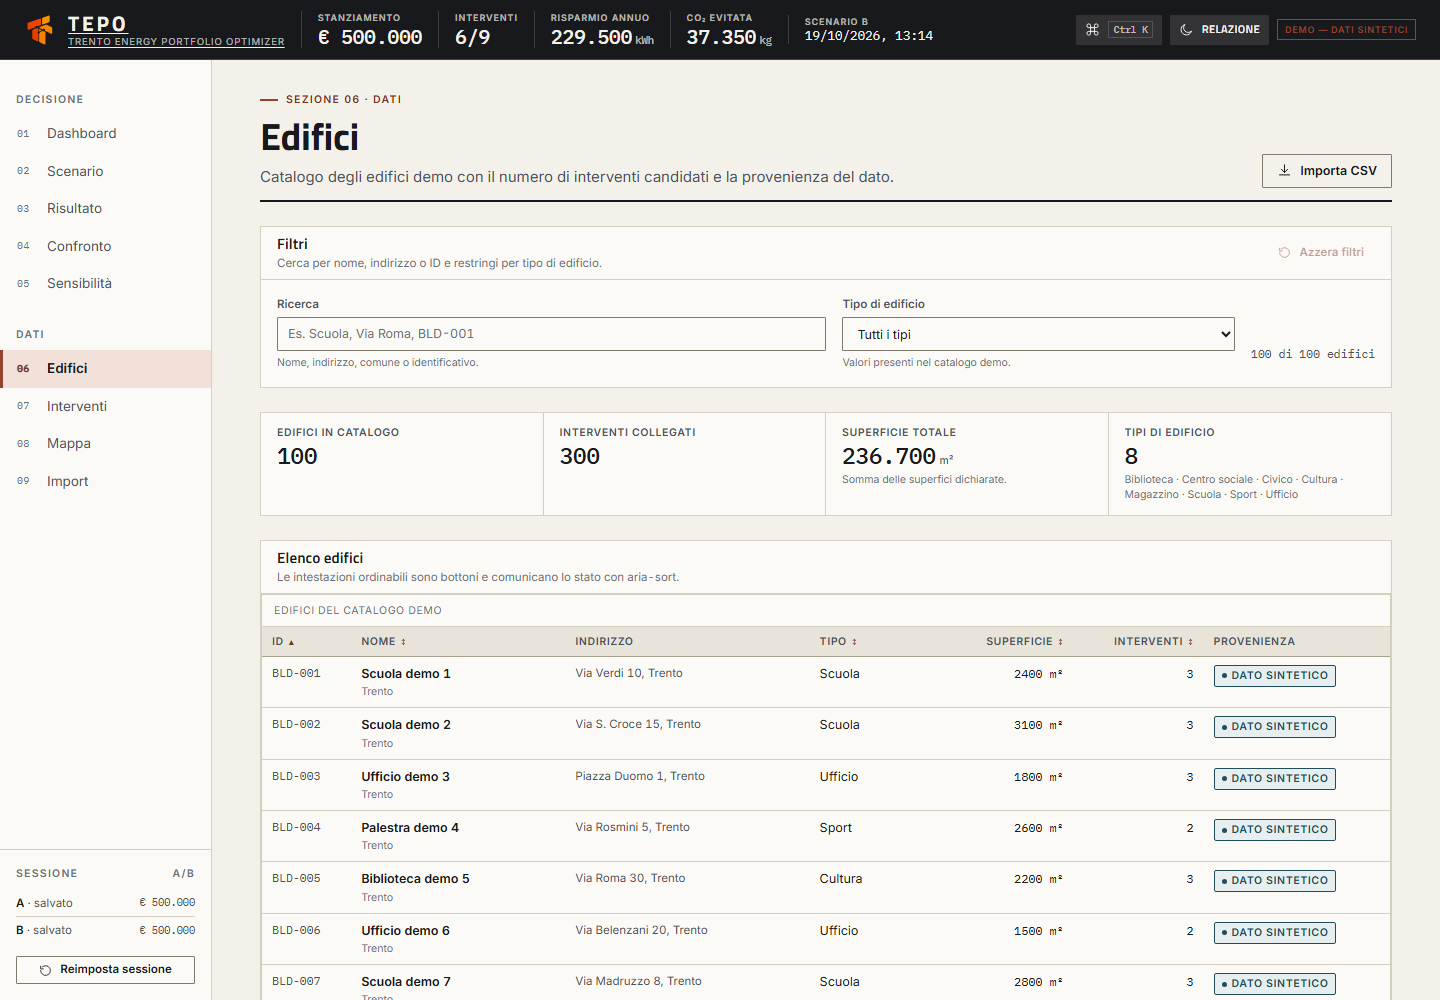
\includegraphics[width=\linewidth]{img/edifici.png}
        \caption{Vista tabellare del catalogo edifici.}
        \label{fig:screen_edifici}
    \end{subfigure}
    \hfill
    \begin{subfigure}[t]{0.48\linewidth}
        \centering
        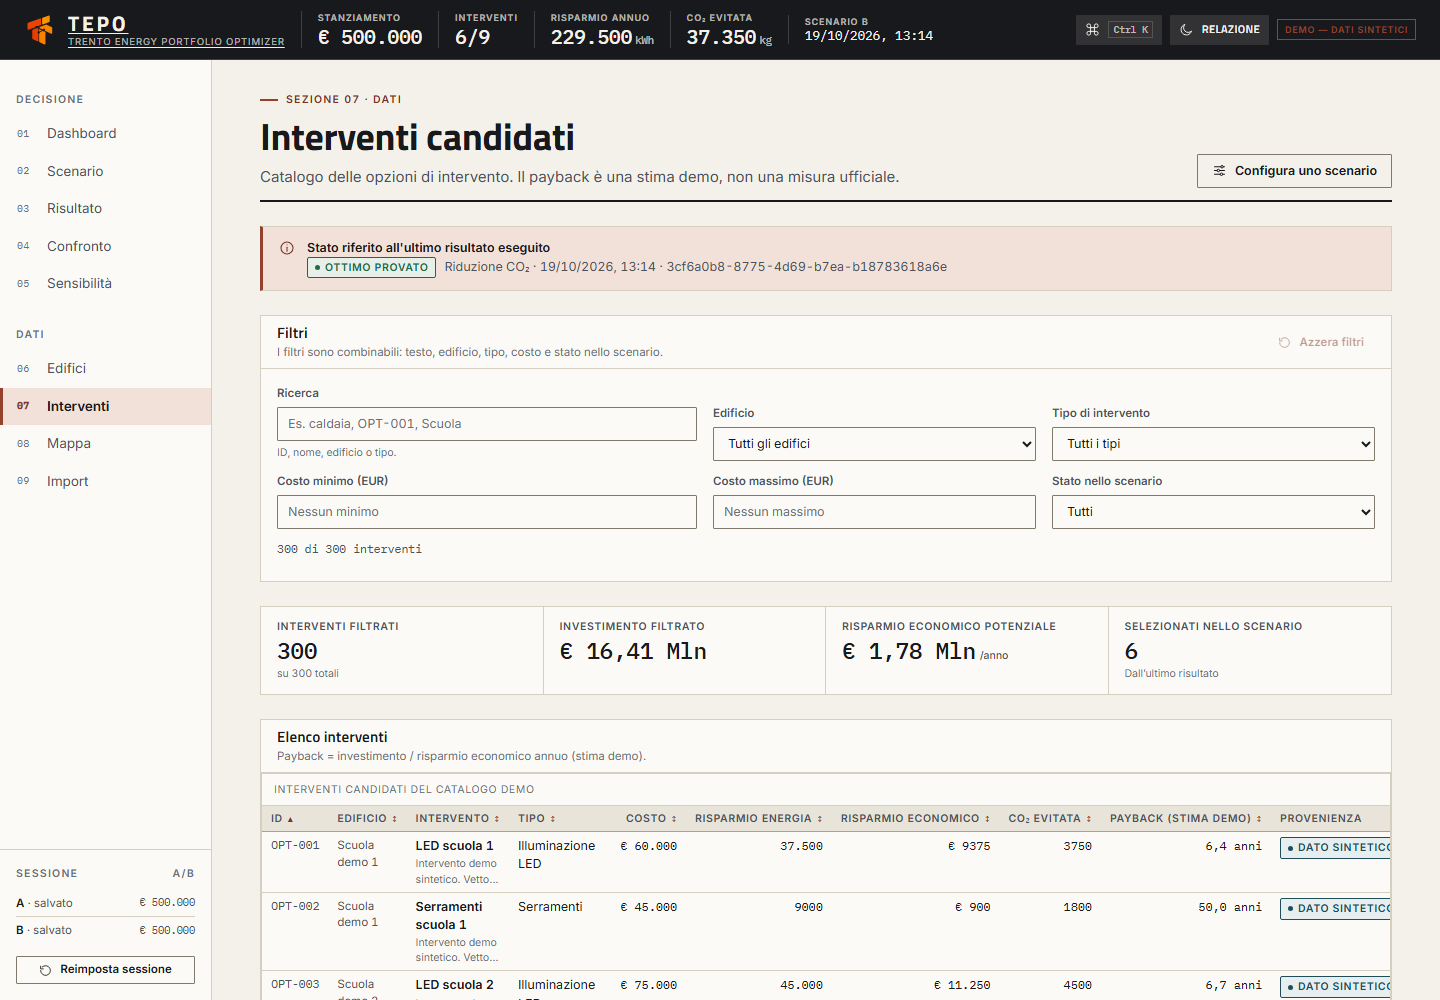
\includegraphics[width=\linewidth]{img/interventi.png}
        \caption{Vista catalogo interventi per tipologia tecnologica.}
        \label{fig:screen_interventi}
    \end{subfigure}
    \caption{Viste di consultazione dei cataloghi comunali.}
    \label{fig:screens_cataloghi}
\end{figure}

\subsubsection{4. Configurazione Scenario (\texttt{ScenarioBuilder})}
La vista \texttt{ScenarioBuilder} (Figura~\ref{fig:screen_scenario}) rappresenta la cabina di regia operativa per l'operatore tecnico:
\begin{itemize}[leftmargin=1.4em, itemsep=0.15em]
    \item \textbf{Parametri Finanziari e Obiettivo:} Cursore numerico per l'impostazione del budget e selezione dell'obiettivo prioritario tra kWh, \euro{} e CO\textsubscript{2};
    \item \textbf{Selezione Candidati:} Selezione rapida per edificio o tipologia con conteggio in tempo reale del budget teorico impegnato;
    \item \textbf{Regole e Vincoli di Policy:} Configurazione di vincoli di mutua esclusione tra interventi, dipendenze tecnologiche di prerequisito e limiti massimi;
    \item \textbf{Pannello Assistente AI:} Modulo a scomparsa per la compilazione guidata da testo naturale con revisione umana.
\end{itemize}

\begin{figure}[H]
    \centering
    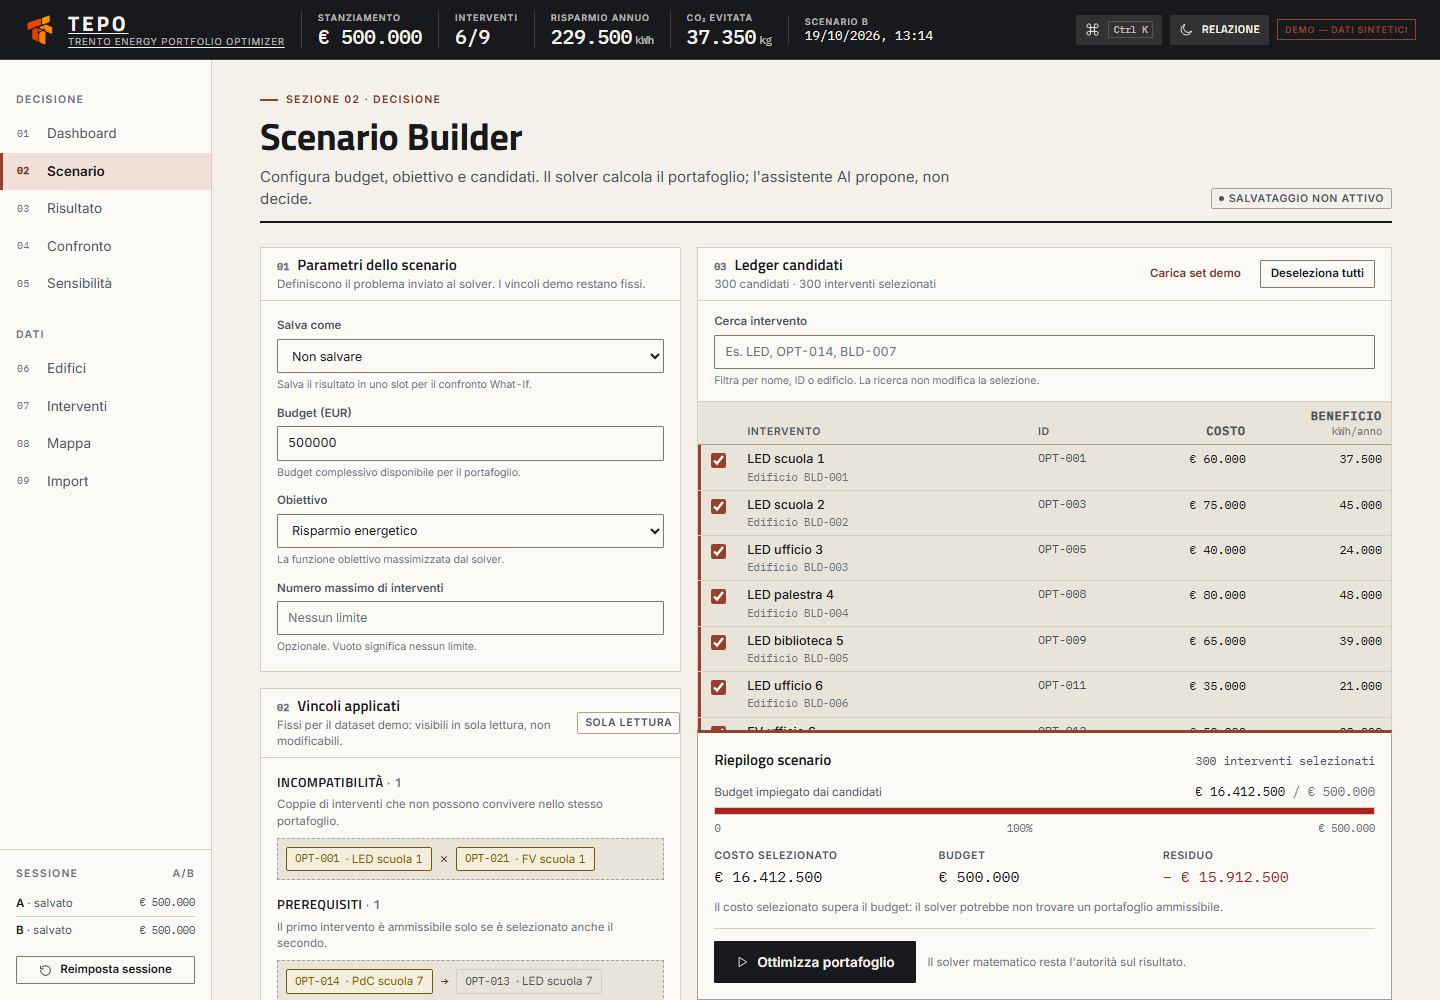
\includegraphics[width=0.85\linewidth]{img/scenario.png}
    \caption{Schermata di configurazione dello scenario decisionale e dei vincoli.}
    \label{fig:screen_scenario}
\end{figure}

\subsubsection{5. Risultato dell'Ottimizzazione ed Esploratore Spiegazioni}
La vista \texttt{ResultPage} (Figura~\ref{fig:screen_risultato}) restituisce l'esito della risoluzione ottima calcolata da OR-Tools CP-SAT.
La schermata presenta un cruscotto superiore con la spesa totale allocata, il budget residuo non speso e il valore massimo dell'obiettivo raggiunto, certificando la prova matematica di ottimalità e riportando l'hash canonico SHA-256 registrato in audit trail.
La sezione inferiore visualizza la tabella completa delle opzioni con il chip di stato (\texttt{Selezionato} / \texttt{Escluso}) e la motivazione deterministica associata calcolata dal motore di spiegazione.

\begin{figure}[H]
    \centering
    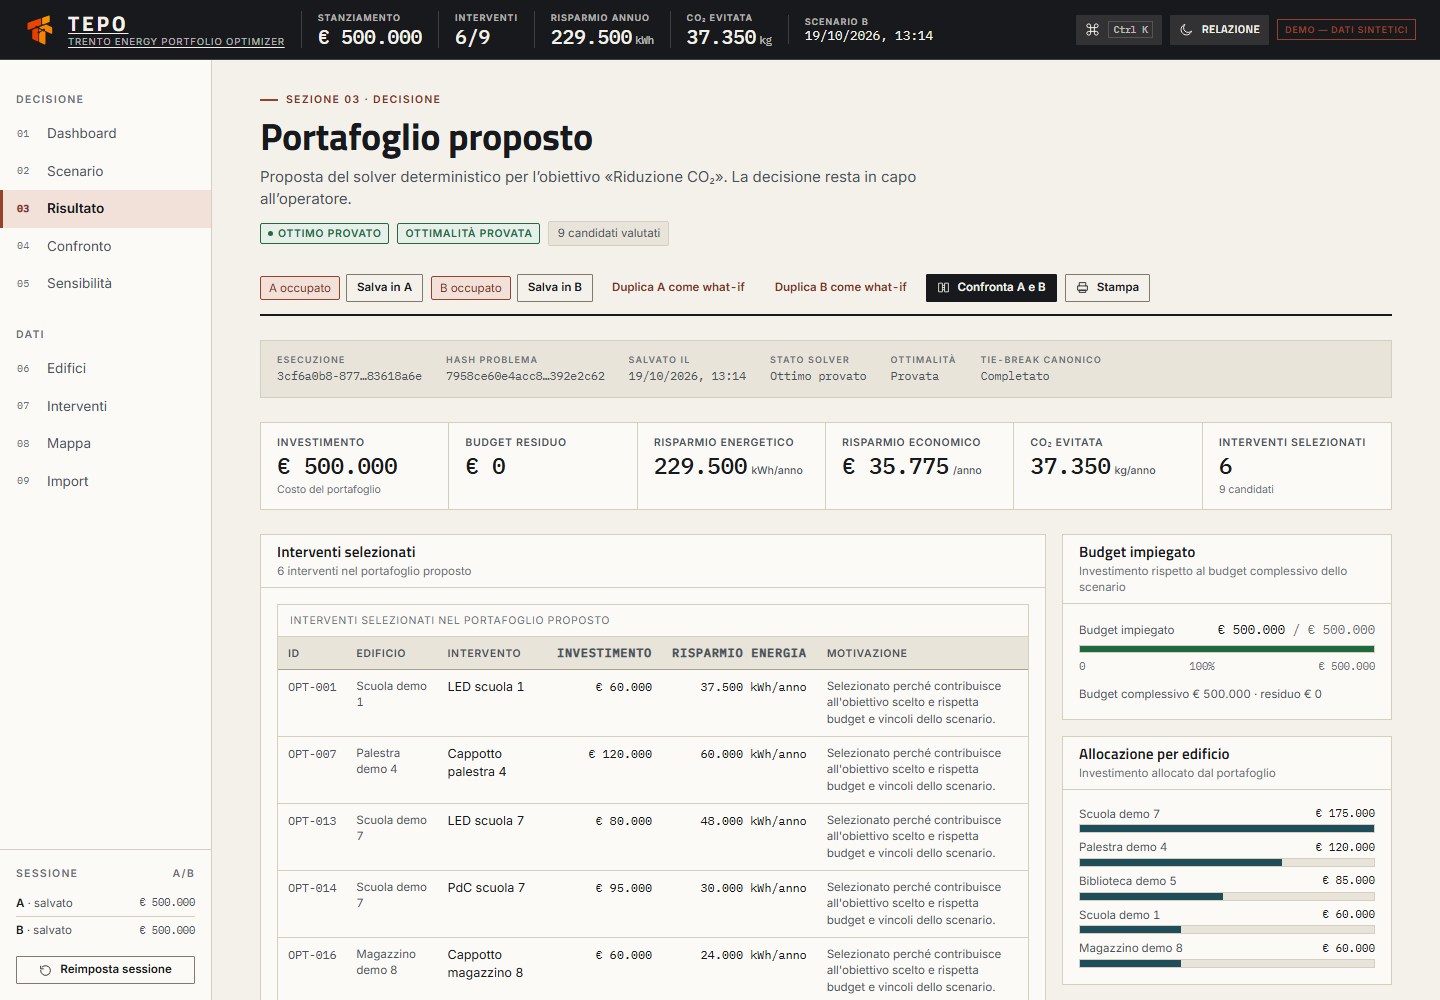
\includegraphics[width=0.88\linewidth]{img/risultato.png}
    \caption{Vista del risultato dell'ottimizzazione con cruscotto KPI e spiegazioni deterministiche.}
    \label{fig:screen_risultato}
\end{figure}

\subsubsection{6. Confronto Scenari What-If (Slot A vs Slot B)}
La vista \texttt{ComparePage} (Figura~\ref{fig:screen_confronto}) affianca due scenari salvati dall'operatore nei due slot di sessione. Il sistema calcola istantaneamente i delta differenziali ($\Delta = \text{B} - \text{A}$) evidenziando con formattazione semantica (verde per miglioramenti, rosso per incrementi di costo o perdite di beneficio) le differenze su investimento complessivo, risparmio energetico, risparmio economico ed emissioni abbattute, permettendo al decisore di comprendere chiaramente il trade-off delle scelte.

\begin{figure}[H]
    \centering
    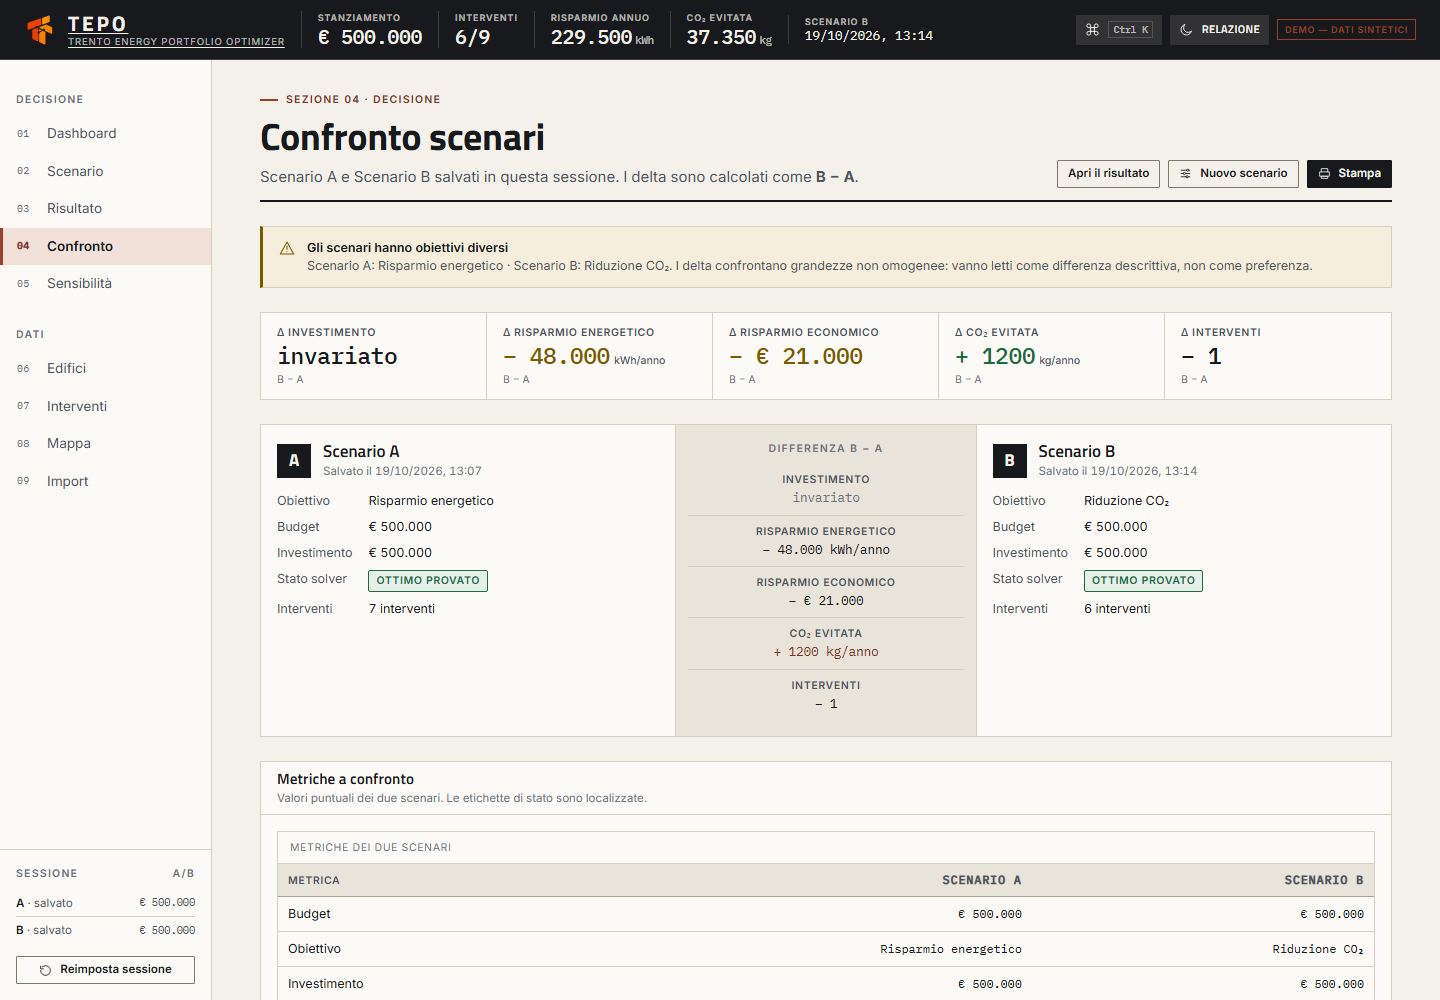
\includegraphics[width=0.85\linewidth]{img/confronto.png}
    \caption{Vista di confronto What-If tra due scenari con calcolo automatico dei differenziali.}
    \label{fig:screen_confronto}
\end{figure}

\subsubsection{7. Analisi di Sensibilità sul Budget}
La vista \texttt{SensitivityPage} (Figura~\ref{fig:screen_sensibilita}) espone i risultati dello sweep parametrico. Un grafico SVG vettoriale visualizza la curva dell'obiettivo in funzione del budget a gradini uniformi, mentre la tabella di stabilità sottostante categorizza le opzioni evidenziando quelle stabili (sempre incluse a qualsiasi budget) rispetto a quelle instabili o fortemente sensibili a scostamenti finanziari minimi.

\begin{figure}[H]
    \centering
    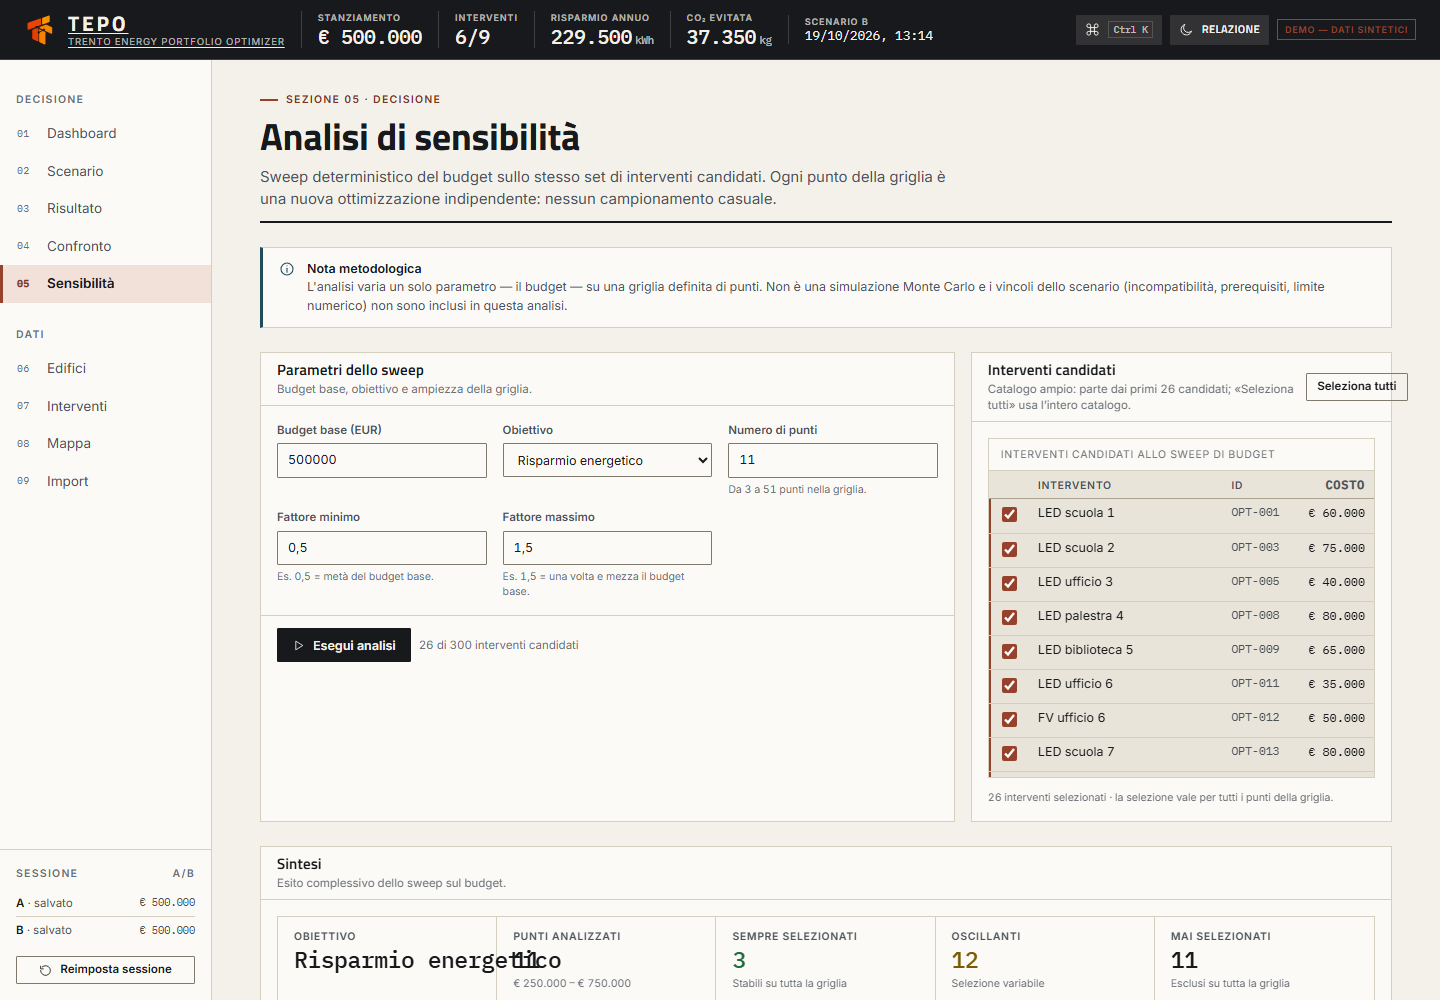
\includegraphics[width=0.85\linewidth]{img/sensibilita.png}
    \caption{Vista dell'analisi di sensibilità parametrica con curve di stabilità e heatmap.}
    \label{fig:screen_sensibilita}
\end{figure}

\subsubsection{8. Importazione Guidata Dati da CSV}
La vista \texttt{ImportPage} (Figura~\ref{fig:screen_import}) guida l'operatore nell'ingestione di file esterni. La schermata mostra l'anteprima delle prime righe, il riepilogo della validazione a secco (segnalando errori di formato, chiavi duplicate o assenza di campi obbligatori) e il pulsante finale di autorizzazione al commit atomico sul database.

\begin{figure}[H]
    \centering
    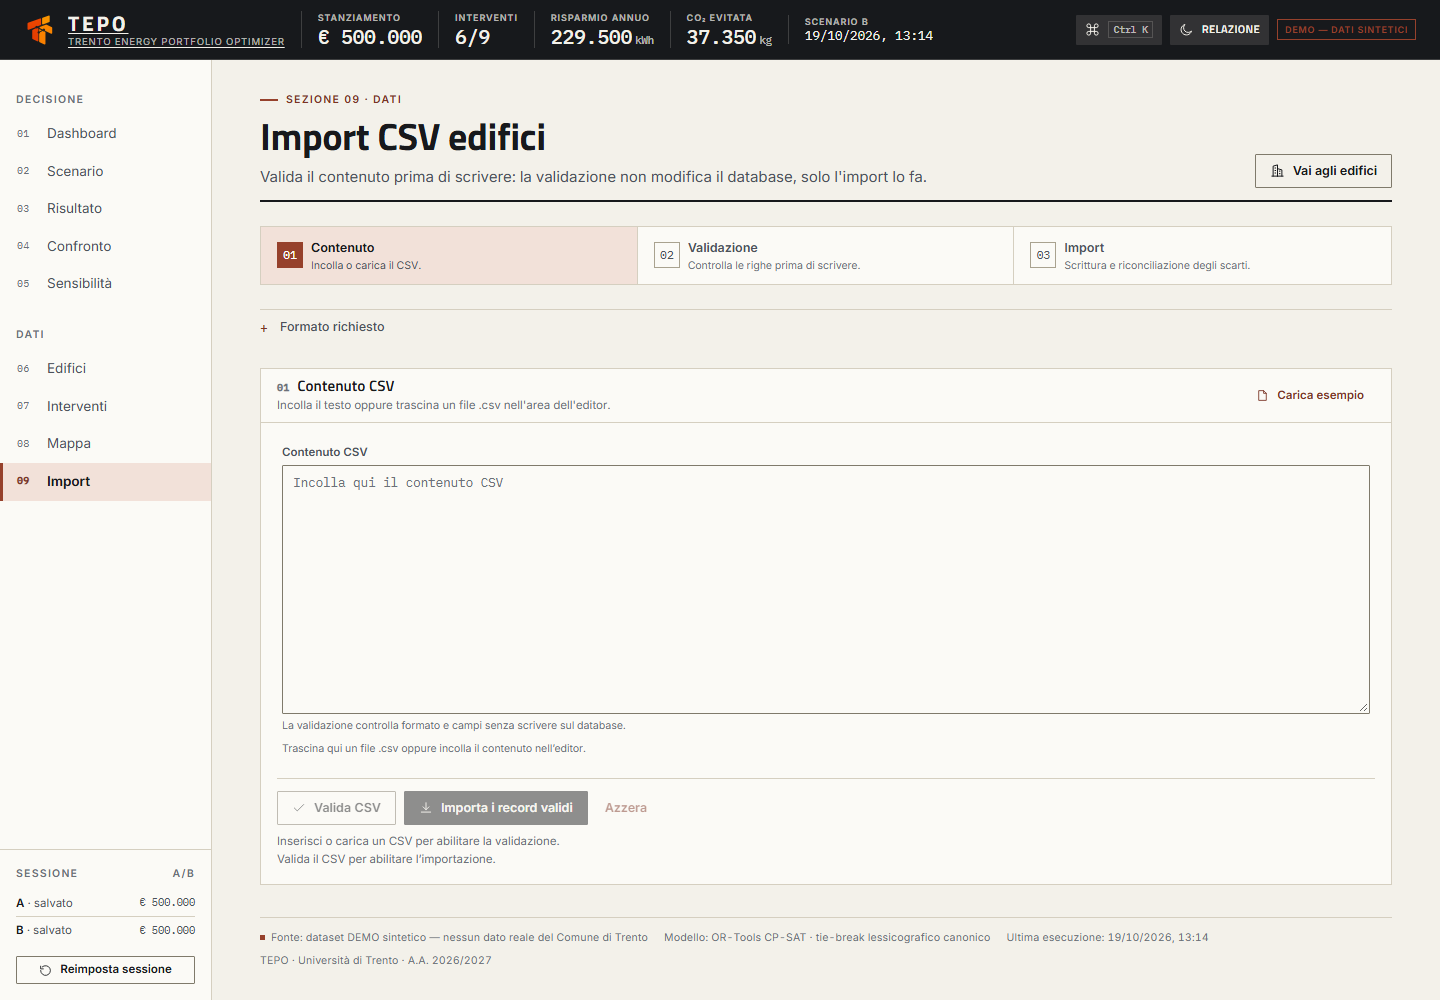
\includegraphics[width=0.85\linewidth]{img/import.png}
    \caption{Procedura guidata in tre passi per l'importazione e validazione dati CSV.}
    \label{fig:screen_import}
\end{figure}
